
\documentclass[a4paper, 11pt]{article}

\usepackage[utf8]{inputenc}
\usepackage[french, english]{babel}
\usepackage[T1]{fontenc}
\usepackage{lmodern}
\usepackage{amsmath}
\usepackage{ccaption}
\usepackage{caption}
\usepackage{chngcntr}
\usepackage{enumitem}
\usepackage{fancyhdr}
\usepackage{float}
\usepackage{gensymb}
\usepackage{geometry}
\usepackage{graphicx}
\usepackage{wrapfig}
\usepackage{hyperref}
\usepackage{lastpage}
\usepackage{layout}
\usepackage{multicol}
\usepackage{multirow}
\usepackage[final]{pdfpages} 
\usepackage{pstricks}
\usepackage{siunitx}
\usepackage{soul}
\usepackage{titlesec}
\usepackage[normalem]{ulem}
\usepackage{url}
\usepackage{xcolor}
\usepackage{colortbl}
\usepackage{setspace}
\usepackage{scalerel}
\usepackage{subfigure}
\usepackage{pythonhighlight}
\usepackage{bm}
\usepackage{svg}


\usepackage[backend=biber, citestyle=authoryear, bibstyle=science]{biblatex}
\appto{\bibsetup}{\raggedright}
\addbibresource{mylib.bib}
\geometry{hmargin=2.5cm,vmargin=2.5cm}
% \geometry{
%   inner=37.125mm,
%   outer=33.4125mm,
%   top=37.125mm,
%   bottom=37.125mm,
%   heightrounded,
%   marginparwidth=51pt,
%   marginparsep=17pt,
%   headsep=24pt,
% }

\fancyhf{}

\newcommand{\Name}{Eyholzer Yannick}
\newcommand{\Title}{PAI project}
%\newcommand{\Title}{\uppercase{Extraction of quasi periodic signals in noisy data using machine learning:\\Application to the detection of exoplanets}}


\newcommand{\todonote}[3] {
	\textbf{\textcolor{#2}{#3 - #1}}
}

\newcommand{\unsurenote}[2] {
	\textbf{\textcolor{#1}{#2}}
}

\newcommand{\todo}[1] {\todonote{TODO}{blue}{#1}}
\newcommand{\note}[1] {\unsurenote{green}{#1}}






\lhead{\ifthenelse{\value{page}=0}{}{\ifthenelse{\value{page}=0}{}{\Name}}}




\chead{\ifthenelse{\value{page}=0}{%page 1
    }{%sinon
        \ifthenelse{\value{page}=0}{%page 1
        }{%sinon
}}}



\rhead{\ifthenelse{\value{page}=0}{%page 1
    }{%sinon
        \ifthenelse{\value{page}=0}{%page 1
        }{%sinon
            \today}}}
\lfoot{\ifthenelse{\value{page}=1}{%page 1
    }{%sinon
}}
\rfoot{\ifthenelse{\value{page}=1}{%page 1
    }{%sinon
    }
}
\cfoot{\ifthenelse{\value{page}=1}{%page 1
        Page \thepage \hspace{1pt} of \pageref*{LastPage}}{%sinon
        \ifthenelse{\value{page}=0}{%page 1
        }{%sinon
            Page \thepage \hspace{1pt} of \pageref*{LastPage}}}}
\setcounter{page}{-1}
\date{\Large{ \today}}



\renewcommand{\headrulewidth}{
    \ifnum\value{page}=0
    0pt
    \else
    \ifnum\value{page}=0
    0pt
    \else
    0.5pt
    \fi
    \fi}

\pagestyle{fancy}









 \begin{document}
    \selectlanguage{english}
    
    
    
    
    %\vspace{6pts}
    
    %\maketitle
    \thispagestyle{empty}       
    \definecolor{light-gray}{gray}{0.90}
    \newcommand{\code}[1]{\colorbox{light-gray}{\texttt{#1}}}
    
    
    \begin{titlepage}
    	
    
%\geometry{hmargin=2.5cm,vmargin=2.5cm}
 \newgeometry{
	   inner=2.5cm,
	   outer=2.5cm,
	   top=2.5cm,
	   bottom=0cm,
	 }
    	
    	\centering
    	\rule{\linewidth}{1mm}
    	%\vspace{6pts} 
    	\huge{\textbf{\Title}} \\
    	\vspace{-3mm}
    	\rule{\linewidth}{1mm}
    	\\[1cm]
    	\large{Yannick Eyholzer}
    	\\[1cm]
    	\large{Physic Application of AI}
    	\\[1cm]
    	
    	\today
    	
%    	\begin{center}  
\includegraphics[width=0.3\linewidth]{images/unilogo.jpg}  
%    	\end{center}
%    	
    	 %\vspace{1cm}
    	
    	\begin{center}  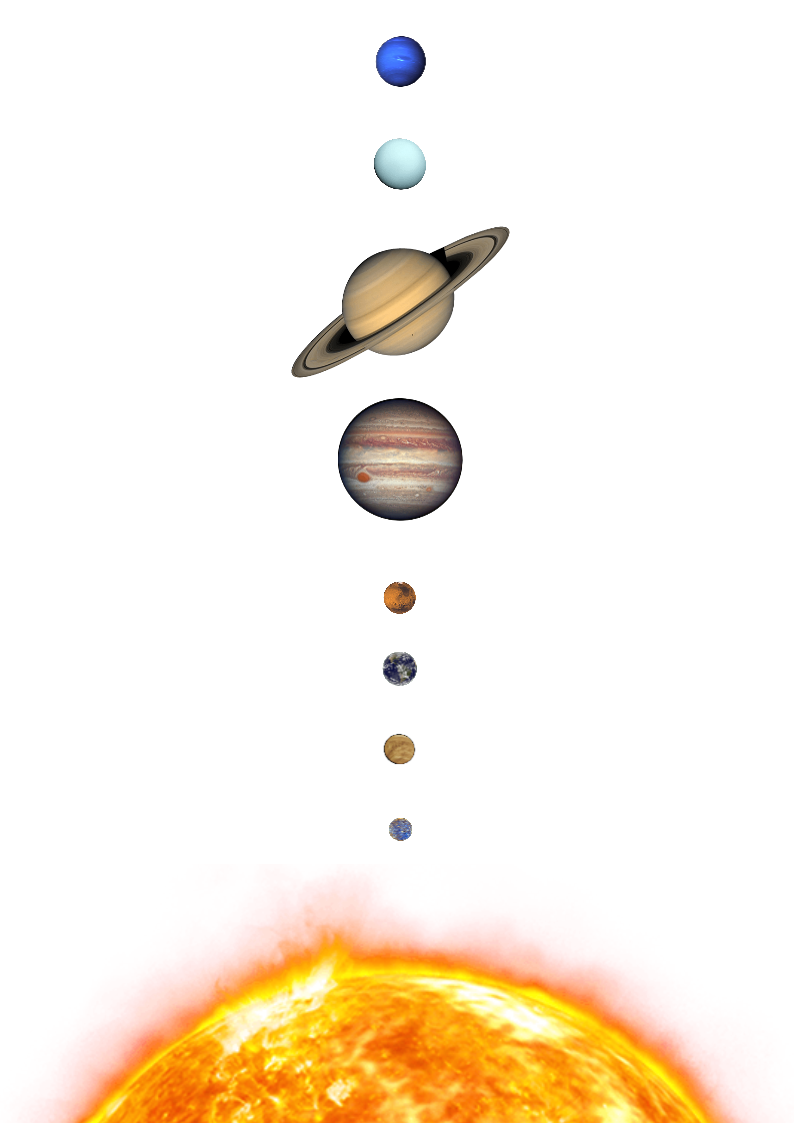
\includegraphics[width=.9\linewidth]{images/solar_system_firstpage.png}  
    	\end{center}
		    	
    	
       
    	\end{titlepage}
    	
    	\restoregeometry
    	
    	\newpage
    	\thispagestyle{empty}       
    	\newpage
    

    \spacing{1.2}
    
    \section{Introduction}
    The goal of the project is to predict the disk features that drives the planet evolutions in the bern model simulations \todo{resume projects}
    
    
    \section{Theory}
   
   
    \subsection{Planet formation and evolution}
    
    \todo{proof read synthax}
    Our understanding of things is always limited by how far we can see. This is specially the case in Astrophysics. Hence our comprehension of planets were for a long time based on the solar system planets.
    
    \begin{figure}[H]                                           
    	\centering 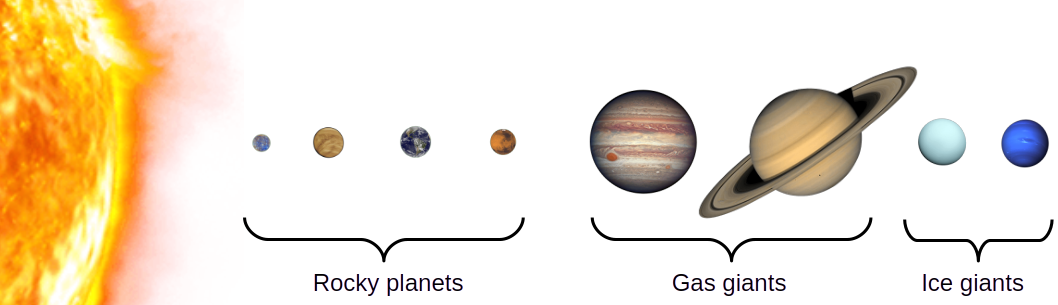
\includegraphics[width=1\textwidth]{images/solar_system_cropped.png}
    	\caption{Representation of the solar system showing each planet sorted by distance: \textit{Mercury}, \textit{Venus}, \textit{Earth}, \textit{Mars}, \textit{Jupiter}, \textit{Saturn}, \textit{Uranus} and \textit{Neptune}. Pluto wishes it was here.}
    	\label{fig:solar_system}
    \end{figure}
    
    From the solar system one can infer three distinct populations: the \textit{rocky planets}, the \textit{gas giants} and the \textit{ice giant}. At the time people started thinking about how would planet outside our solar system - extrasolar planets or exoplanet - look like, it was natural to expect them to look like the one from our solar system.  A pletora of different formation models and hypothesis for planets emerged with time. Philosopher, mathematician and astrophysicist worked hard building new theories on top of old ones, discarding proven wrong aspect and keeping the good ones, to result in a theory close to the contemporary one; the nebular hypothesis. 
    
    The nebular hypothesis states that solar systems form from the collapse of a giant nebular cloud, being an enormous quantity of gas spanning multiples light years floating in the galaxy. Some external perturbation such as a close supernovae, a close encounter or collision with another cloud would cause the gravitational collapse of the nebular cloud. Most of the mass of the cloud would form the star at the center, and the residual matter would flattened into the protoplanetary disk around the star. Every other celestial bodies such as the planets would form from this disk. 
    
    Following this model, gas and ice giant would form in the disk at a distance that is far enough to the star to have solid water. Ice helping the accretion of mass, these planet can acrete more mass thus becoming bigger. This delimitation between solid and liquid water is called the ice line. Before the ice line, the water being liquid and gaseous, the planets forming there are less capable of acreting mass thus being smaller. This is were the rocky planets form. This model fits well the current hierarchical architecture of our solar system, visible in figure \ref{fig:solar_system}.
    
    
    
   	One can imagine the effect on the scientific community of discovering the first exoplanet around a star similar to the sun being a Jupiter-sized planet 10x closer to the sun than Earth, visible as the red dot on the left of figure \ref{fig:mass_distance_cropped}. According to the model at the time, this was impossible. Thus the discovery was first highly criticizing and received with scepticism, but end up rewarding the Nobel prize to Michel Mayor and Didier Queloz for being the first exoplanet around a sun-like star discovered. Later on, a lot more of exoplanets have been detected with different methods, visible on the right of figure \ref{fig:mass_distance_cropped}. These new discoveries, even thought they are bias toward easy discoverable planets, shows that our solar system may not represent the norm of solar systems.
   	  \begin{figure}[H]                                           
   		\centering 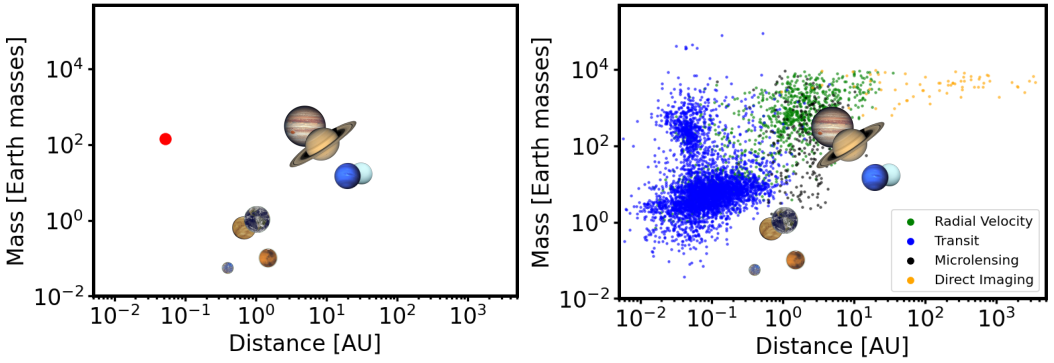
\includegraphics[width=1\textwidth]{images/mass_distance_cropped.png}
   		\caption{Plots of the distance of the planet to the host star in astronomical unit (AU) (Earth is at 1 AU) as a function of the mass of the planet in Earth mass.  The left plot shows the solar system planets with the first discovered Jupiter like planet in red.  The right plots adds the current exoplanets detected for a selection of the best 4 methods.}
   		\label{fig:mass_distance_cropped}
   	\end{figure}
   	
   
   	
   	The main drawback in the creation of good planetary models and better understanding in astronomy is the enormous distance and timescale we are dealing with.  On the scale of their life, we observe snapshot of systems which light took a few years to hundred of thousand of years to reach us. We cannot observe a system from birth to death, as solar systems probably form for at least Million of year and keep on living until the supernovae of the host star up to Billion of years later.  Finally, the relative size and brightness of the planets compared to their host star make them hard to detect, and even harder to completely characterize a solar system.
   	
   	These obstacles motivated astronomer to develop simulations in addition to the observations and theory already used. These simulations would be based on models, and the results would be compared to observations that would allow to verify how good the model is. They would allow to "observe" a system and their planet during their complete lifespan, to test different formation and evolution mechanism.
    
    
    \subsection{Bern model}
 	The bern model  \todo{cite model} is a simulation process that start from a protoplanetary disk around a star with planetary embryos and simulates the evolutions of the embryos within the disk forming planets. The simulations have been updated multiple times, being more complex each time.  It takes into account chemical,  gravitational  and hydrodynamical process, with N-body interactions. \todo{check bern model paper}
 	\begin{figure}[H]                                           
 		\centering 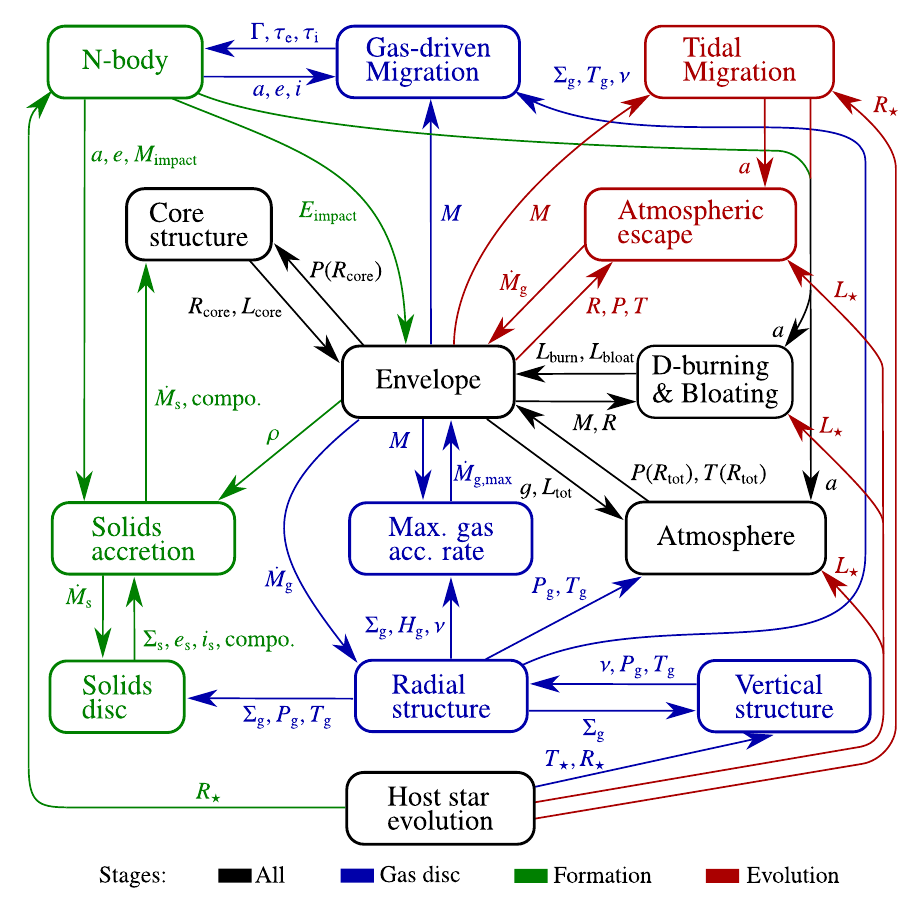
\includegraphics[width=0.5\textwidth]{images/bern_model_schematics.png}
 		\caption{bern model \todo{comment}}
 		\label{fig:bern_model}
 	\end{figure}
 	 
    \section{Goal \& Method}
    
    The goal of the project will be to use result of bern model simulations  to predict the disk characteristics that are driving the planet formations and evolutions. The approach will be to train a model on the disks feature and to use the resulting formed planet as targets. Then, to determine the features driving the planet formations, the feature importances will be determined.
    
    \subsection{The raw dataset}
    The dataset is the results of bern model simulations for a host star of 1 solar mass, with the evolution of a total of 15'000 disks containing each 20 planetary embryos initially. The dataset posses information on the disk initial condition of the simulation and the characteristics of each planets resulting from the evolution of the disk. that are still in the system.
    
    The disk properties are: 
      \begin{itemize}
      	  \setlength\itemsep{-.2em}
      	\item \textit{Metallicity}
      	\item \textit{Gas disk (Msun)}
      	\item \textit{Solid disk (Mearth)}
      	\item \textit{life time (yr)}
      	\item \textit{luminosity}
      \end{itemize}
      
    The propoerties of each planet are:
    \begin{itemize}
    	\setlength\itemsep{-.2em}
    	\item \textit{The total mass (Mearth)}
    	\item \textit{The semi major axis (AU)}
    	\item \textit{the gas to core ratio}
    	\item \textit{the fraction of water}
    	\item \textit{the initial semi major axis} at the beggining of the simulation
    	\item \textit{the radius}
    \end{itemize}
    
    
    \subsection{Processing the dataset}
    
    \subsubsection{Disk features}
    Looking at the distribution of the disk features in figure \ref{fig:disk_feature_distribution}, we can see some typical right-skewed distribution. This non-uniformity in the distribution of the features can affect the learning and generalisation capacity of the models, thus a change of representation can be useful. Looking at the figure  \ref{fig:disk_feature_log_distribution}, we can see that the log10 scale is a good choice. This is the representation we will use to train the model with.
    
    \begin{figure}[H]                                           
    	\centering 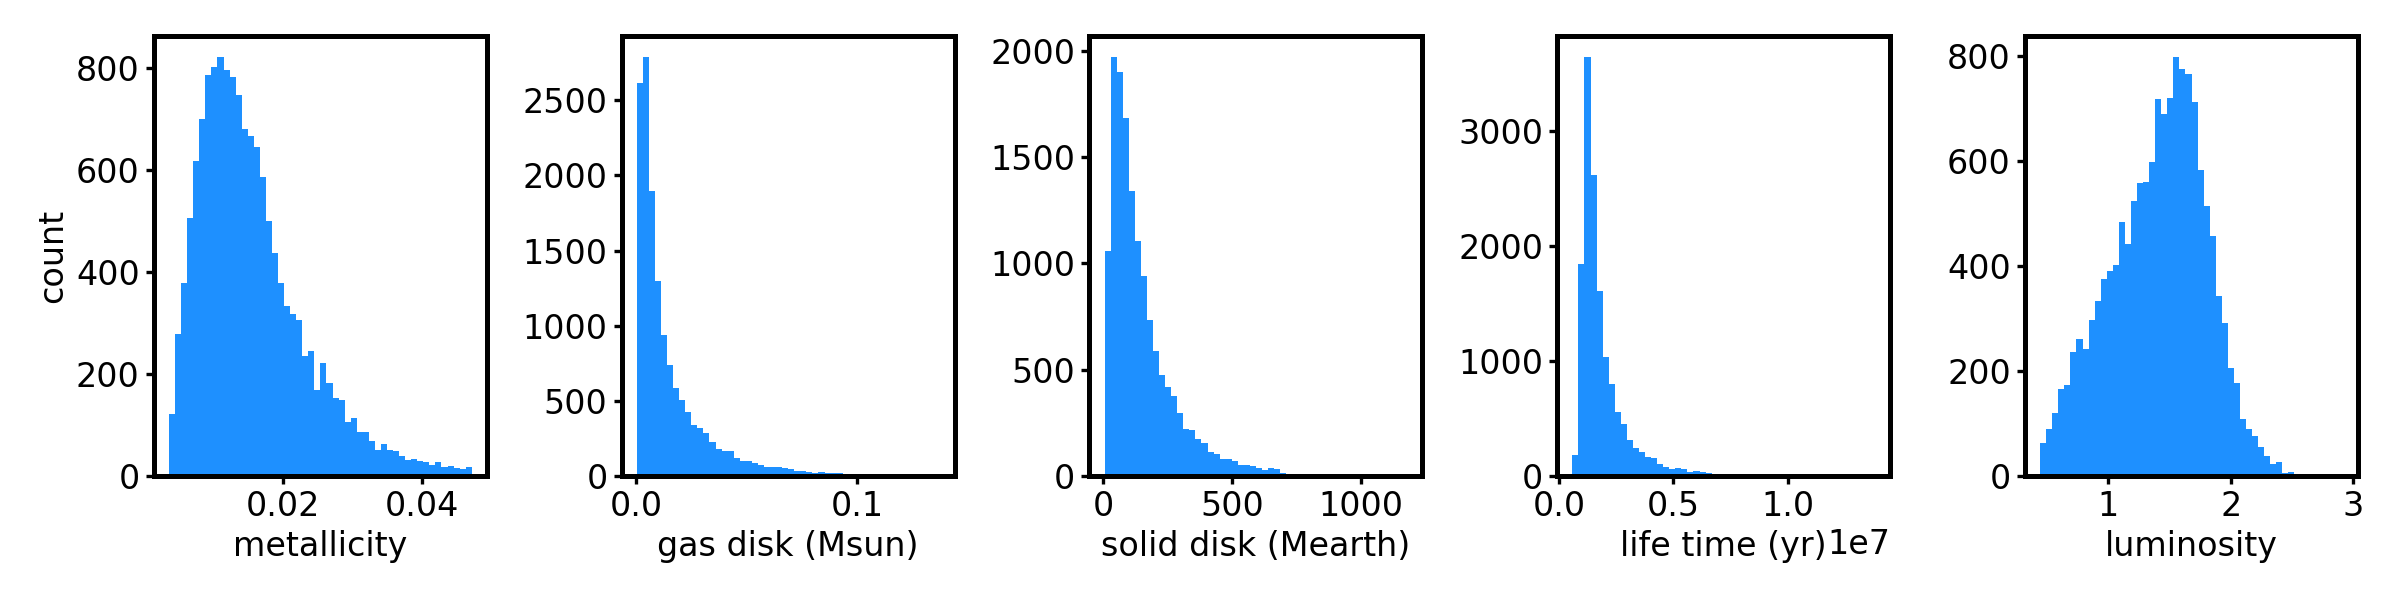
\includegraphics[width=1\textwidth]{images/disk_features_distribution.png}
    	\caption{Distribution of the disk features}
    	\label{fig:disk_feature_distribution}
    \end{figure}
    
    \begin{figure}[H]                                           
    	\centering 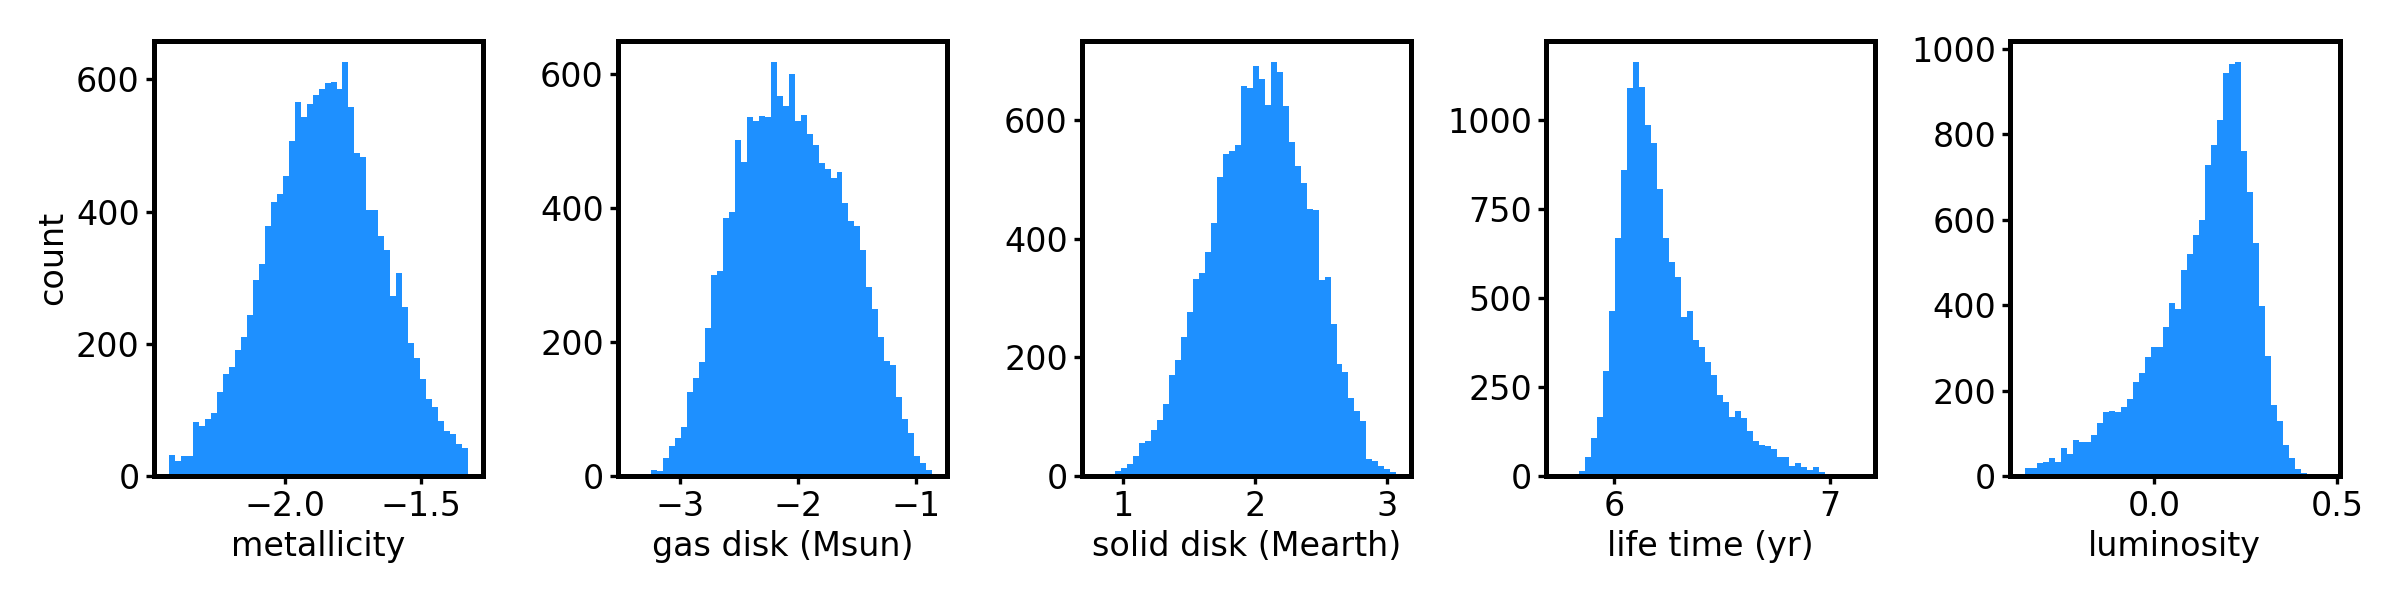
\includegraphics[width=1\textwidth]{images/disk_features_log_distribution.png}
    	\caption{Distribution of the disk features in log10 scale}
    	\label{fig:disk_feature_log_distribution}
    \end{figure}
    
    \subsubsection{Planet features}
    
    The first step with the planets properties is to address the variable number of planets for different disk. As each disk does not necessarily produce the same number of planet, some collide, merge, or are ejected.  In addition to the variable number of planet, their occurrences are not orderer.  Hence the input is constant and ordered, as each disk possesses the same number of features, but the target are variable in size and non-ordered. \todo{two sol: model special or generalization of target}
    
    
    
    \subsection{The models}
    
    The model used 
    
    \subsection{Important features}
    
    To retrieve the feature that are important in the evolution of the planets, we can retrieve the feature importances. In this project two methods are used.
    
    The first method is to use feature permutation. The model is normally trained on the data, then it is tested on a test dataset were the feature of the disks have been permuted \textit{between the disks}. Thus the model will have to predict the target based on disks that have have one of their feature exchanged with all the other disks. For each feature, the permutation is applied and then the performance are measured, and finally we can analyse which feature affected the performance the most, which should be the most important feature.
    
    The second method is to add linear layer at the beggining of the neural network that is connected in a 1-to-1 manner, each input connects to one neurone. Thus, this is possible to analyse the weight of this layer to see which input the model weighted the most as "most important".
    \section{Results}
    
    \subsection{Architecture and  parameters explorations}
       
    \subsubsection{lr test}
    
    The first test to do is to see how the learning rate affects the efficiency of the model, as higher learning rate would allow to train the model for a shorter time. This test was done for 3 differents architectures with a learning rate going from 5e-5 to 1e-1
    
    \subsubsection{batchsize test}
    
    
    \subsubsection{deep test}
    
    \subsubsection{depth test}
    
    
    
    \subsection{Feature importances}
    
    
    
    \section{Conclusion}
    
    
    \end{document}











Tableau:\
\begin{table}[H]
    \centering
    \begin{tabular}{|c|c|c|}\hline
        &&  \\ \hline
        &&  \\
        &&  \\
        \hline
    \end{tabular}
    \caption{XX}
\end{table}\\


Double Tableau:\
\begin{table}[H]
    \begin{minipage}[t]{.4\linewidth}
        \centering
        \begin{tabular}{|c|c|c|c|}\hline
            &&&\\ \hline
            &&&\\
            &&&\\
            &&&\\
            \hline
        \end{tabular}
        \caption{XX}
    \end{minipage}
    \hfill
    \begin{minipage}[t]{.4\linewidth}
        \begin{tabular}{|c|c|c|c|}
            \multicolumn{4}{c}{XX} \\ \hline
            &&& \\ \hline
            &&& \\
            &&& \\
            &&& \\
            \hline
        \end{tabular}
        \caption{XX}
    \end{minipage}
\end{table}


Inclure image:\
\begin{figure}[H]                                           
    \centering \includegraphics[width=0.5\textwidth]{images/.jpg}
    \caption{}
\end{figure}


Double image:\
\begin{figure}[H]
    \begin{minipage}[t]{.4\linewidth}
        \centering 
        \includegraphics[width=0.5\textwidth]{images/.png}
        \caption{}
    \end{minipage}
    \hfill
    \begin{minipage}[t]{.4\linewidth}
        \centering 
        \includegraphics[width=0.5\textwidth]{images/.png}
        \caption{}
    \end{minipage}
\end{figure}

sub image:
\begin{figure}
    \centering
    \begin{subfigure}[b]{0.3\textwidth}
        \includegraphics[width=\textwidth]{image}
        \caption{texte}
        %\label{fig:gull}
    \end{subfigure}
    ~ %add desired spacing between images, e. g. ~, \quad, \qquad, \hfill etc. 
    %(or a blank line to force the subfigure onto a new line)
    \begin{subfigure}[b]{0.3\textwidth}
        \includegraphics[width=\textwidth]{image}
        \caption{texte}
        %\label{fig:tiger}
    \end{subfigure}
    ~ %add desired spacing between images, e. g. ~, \quad, \qquad, \hfill etc. 
    %(or a blank line to force the subfigure onto a new line)
    \begin{subfigure}[b]{0.3\textwidth}
        \includegraphics[width=\textwidth]{image}
        \caption{texte}
        %\label{fig:mouse}
    \end{subfigure}
    %\caption{figure texte}\label{fig:animals}
\end{figure}

